\documentclass[a4paper,11pt,UTF8]{article}
\usepackage{ctex}
\usepackage{amsmath,amsthm,amssymb,amsfonts}
\usepackage{amsmath}
\usepackage[a4paper]{geometry}
\usepackage{graphicx}
\usepackage{microtype}
\usepackage{siunitx}
\usepackage{booktabs}
\usepackage[colorlinks=false, pdfborder={0 0 0}]{hyperref}
\usepackage{cleveref}
\usepackage{esint} 
\usepackage{graphicx}
\usepackage{ragged2e}
\usepackage{pifont}
\usepackage{extarrows}
\usepackage{mathptmx}
\usepackage{float}
\usepackage{caption}
\usepackage{multirow}
\usepackage{subfigure}
\usepackage{titlesec}
\titleformat{\section}{\Large\bfseries}{\chinese{section}、}{0em}{}
\titleformat{\subsection}{\large\bfseries}{\thesubsection}{0em}{}
\titleformat{\subsubsection}{\normalsize\bfseries}{\thesubsubsection}{1em}{}
\begin{document}
	
\begin{titlepage}
	\begin{center}
		\vspace*{1cm}
		\textbf{\Huge 实验报告:集成运算放大器在信号运算方面的应用}
		
		\vspace{0.5cm}
		\Large 谢悦晋\quad 提高2201班\quad U20221033
		
		\vspace{1cm}
		\begin{figure}[H]
			\centering
			\subfigure{
				
\includegraphics[scale=1]{hust}
			}
			\subfigure{
				
\includegraphics[scale=1]{eic}
			}
			\caption*{}
		\end{figure}
		\vfill
		
		
		\vspace{0.8cm}
		华中科技大学 \\
		电子信息与通信学院 \\
		Oct 22nd, 2023
	\end{center}
\end{titlepage}
\tableofcontents
\section{实验目的}
熟练安装、调试本节介绍的由运放构成的基本运算电路,熟练掌握它们的工作原理,掌握运放电路的基本分析
\section{实验器材}
运算放大器NE5532,100$\mathrm{\Omega}$电阻,500$\mathrm{\Omega}$电阻,1$\mathrm{k\Omega}$电阻,5.1$\mathrm{k\Omega}$电阻,10$\mathrm{k\Omega}$电阻,100$\mathrm{k\Omega}$电阻,示波器,信号源,稳压电源
\section{实验内容}
\subsection{任务1: 研究电压跟随器的作用}
测试下图所示两种电路各电压幅值,观察有、无电压跟随器的差别。
\subsubsection{实验电路:}
\begin{figure}[H]
	\centering
	\setcounter{subfigure}{0}
	\subfigure[直接连接]{
		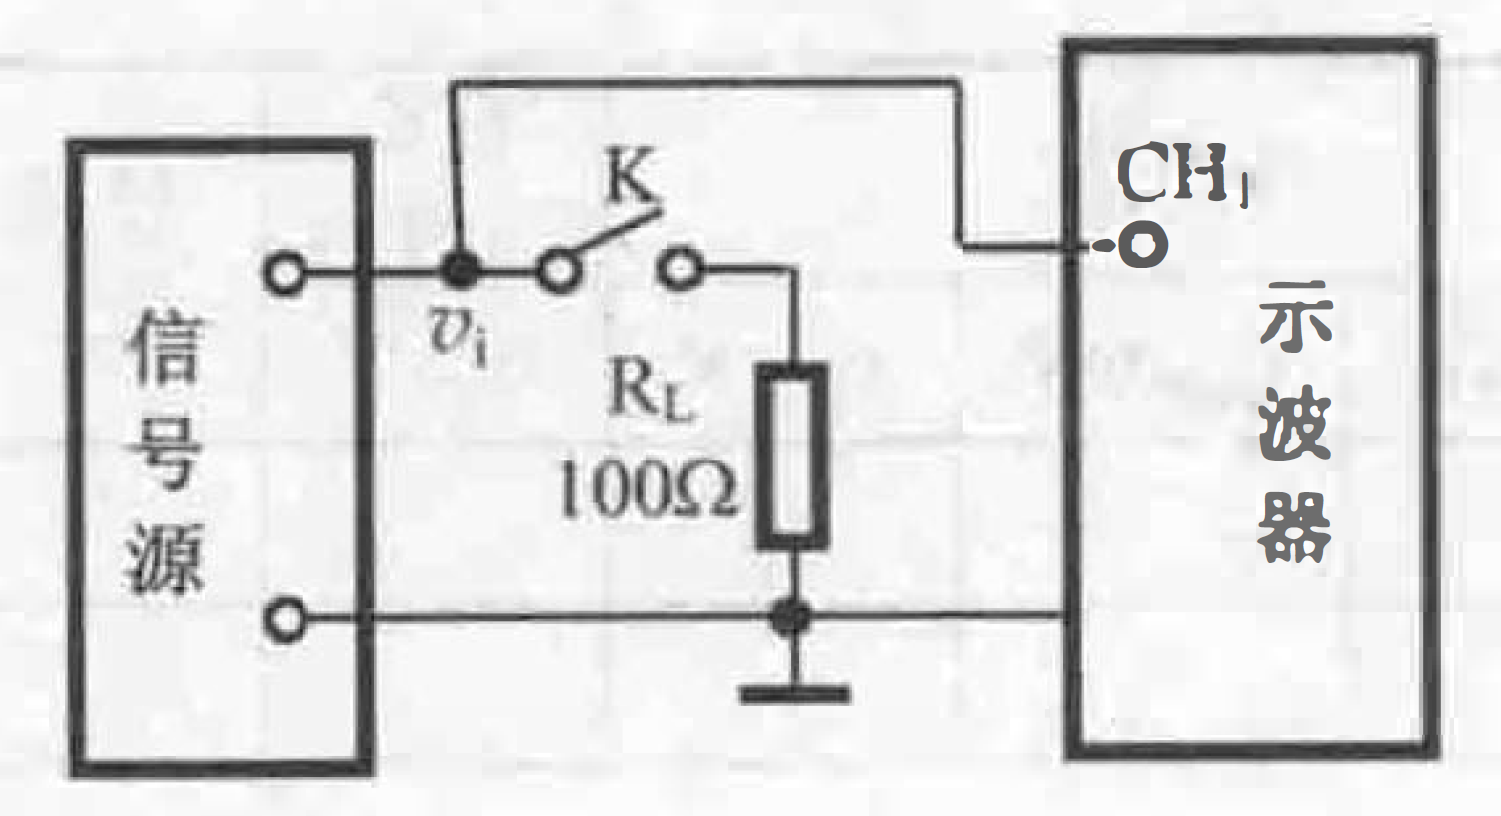
\includegraphics[scale=0.1]{1.1}
		\label{fig:subfig1}		
	}
	\subfigure[通过电压跟随器连接]{
		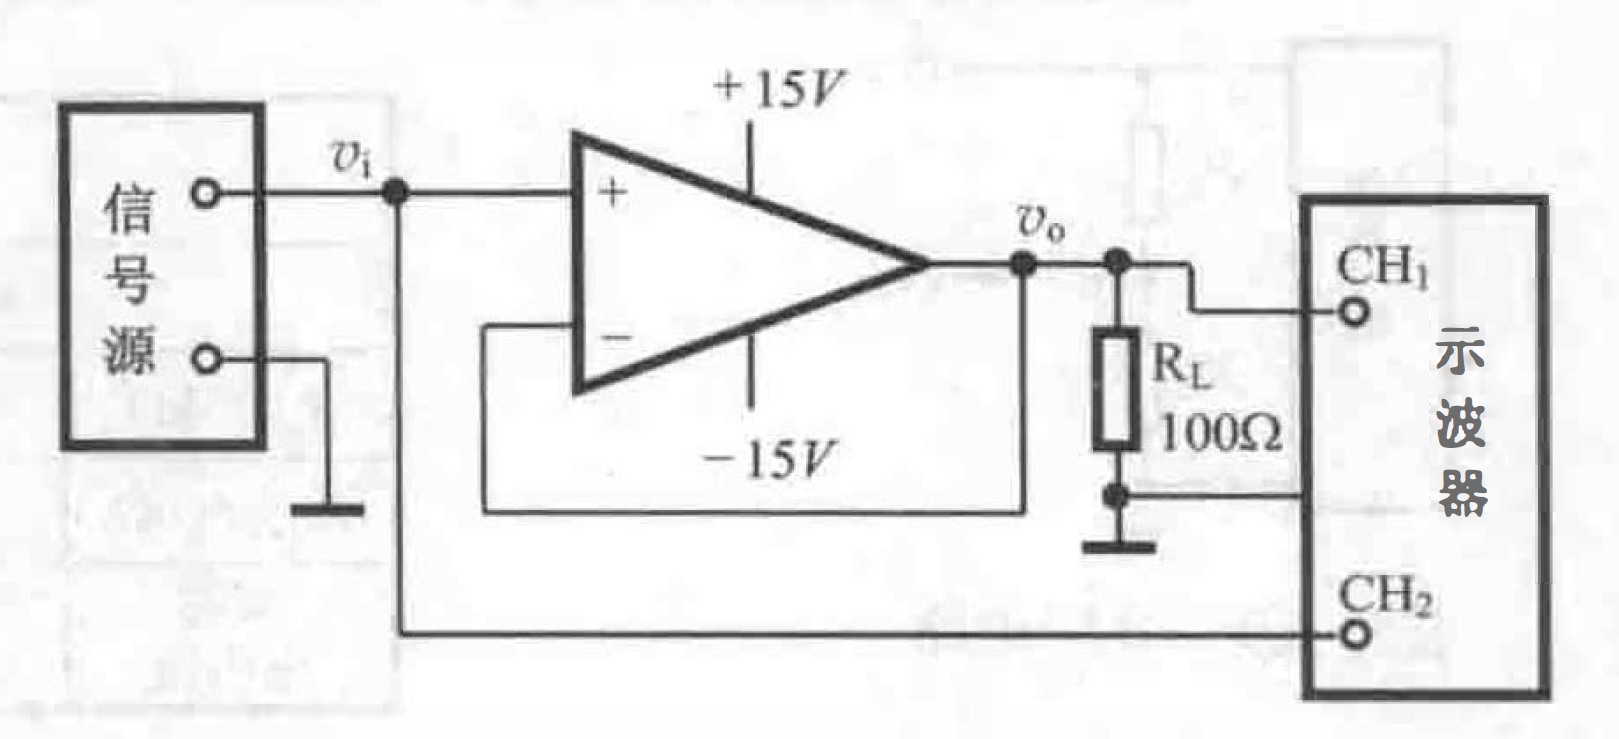
\includegraphics[scale=0.12]{1.2}
	}
	\caption*{任务1: 研究电压跟随器的作用}
\end{figure}
(1)从信号源送出频率为1kHz、峰-峰值为1V的正弦信号。不接负载$R_L$(K断开)时,用示波器观测$v_i$波形并填入下表中;接入负载$R_L$(K闭合)时,用示波器观测$v_i$波形并填入下表中。

(2)按照图(b)连接电路,仍从信号源送出频率为1kHz、峰-峰值为1V的正弦信号,用示波器两个通道同时观察输入、输出波形,分别测量未接$R_L$和接入$R_L$两种情况下$v_i$和$v_io$的大小并填入下表中。

(3)计算信号源的内阻$R_S$,说明100$\Omega$负载电阻连接到信号源上产生的负载效应,并解释观察到的实验现象。
\begin{figure}[H]
	\centering
	\caption*{电压跟随器的作用数据记录表格}
	
	\begin{tabular}{|c|c|c|c|c|c|}
		\hline
		\multirow{2}{*}{}   & \multicolumn{2}{c|}{不接$R_L$} & \multicolumn{2}{c|}{接入$R_L$} &
		\multirow{2}{*}{计算$R_s/\Omega$}\\
		\cline{2-5}
		\multirow{2}{*}{} & $v_{ipp}/$V & $v_{opp}/$V & $v_{ipp}/$V & $v_{opp}/$V & \multirow{2}{*}{}\\
		\hline
		无电压跟随器 &  & - &  & - &  \\
		\hline
		有电压跟随器 &  &  &  &  & - \\
		\hline
	\end{tabular}
	\label{table_MAP}
\end{figure}
信号源的内阻计算可以按照分压公式计算:
$$
	R_s=\frac{V_s-v_{ipp(R_L)}}{v_{ipp(R_L)}}R_L
$$

\subsection{任务2: 反相比例加法运算电路测试}
测试图3.6.8所示反相比例加法器的输入输出电压,验证它们的运算关系。根据运放的虚短和虚断特性,可求得其输出电压为:
$$
	V_0=-\left(\frac{R_{\mathrm{F}}}{R_1}V_1+\frac{R_{\mathrm{F}}}{R_2}V_2\right)
$$
\begin{figure}[H]
	\centering
	\subfigure[分压电路]{
		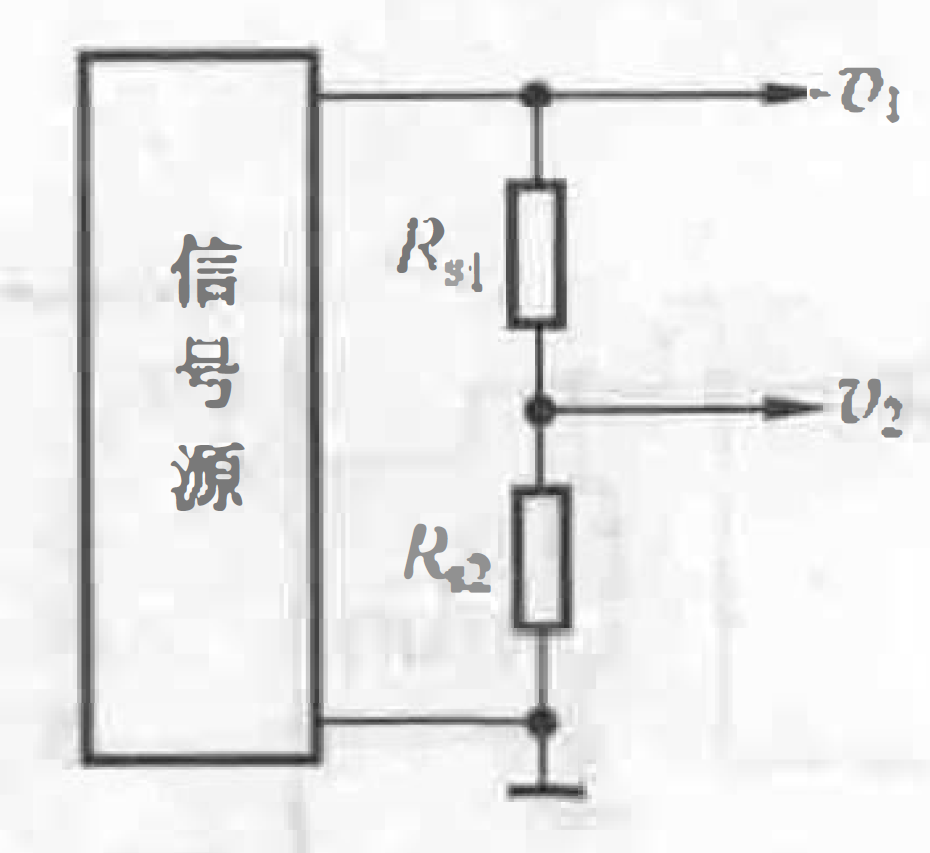
\includegraphics[width=0.48\textwidth]{1.13}
	}
	\subfigure[实验电路图]{
		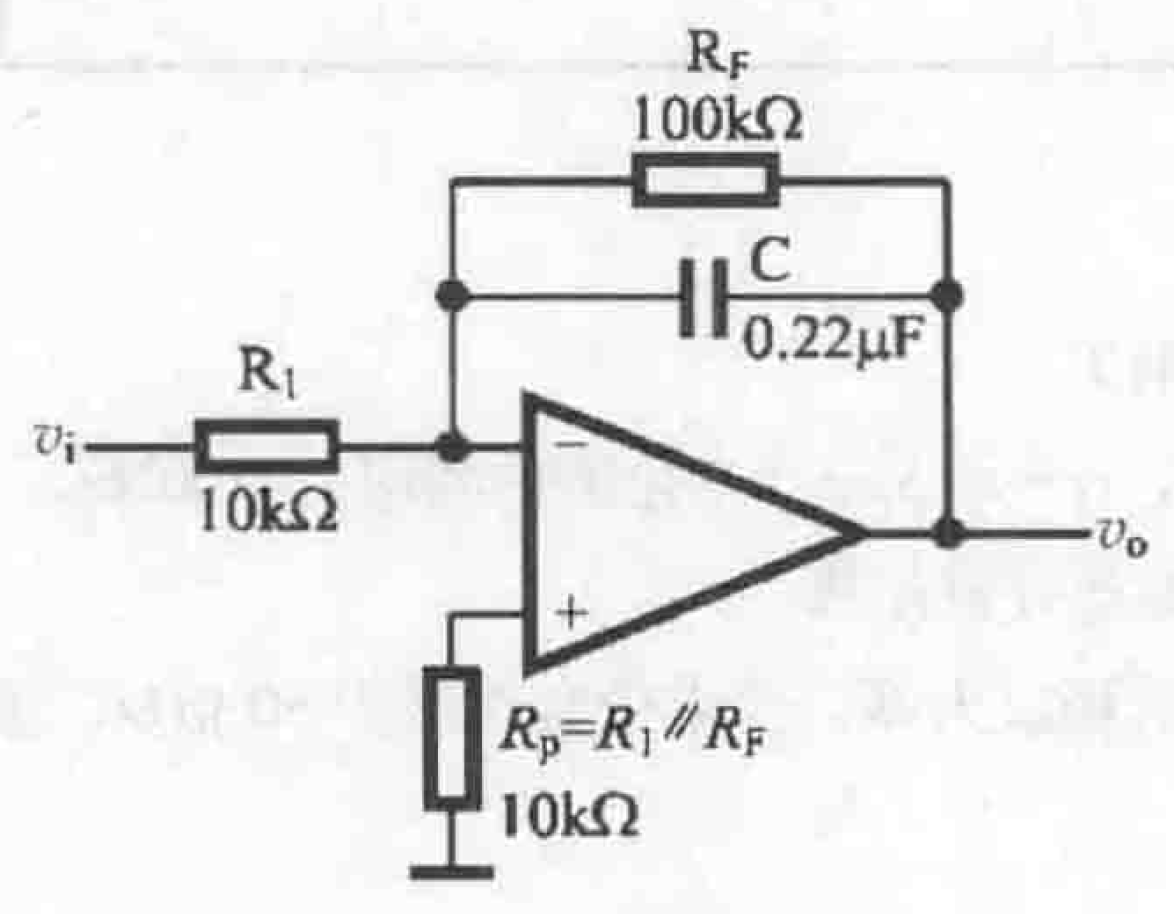
\includegraphics[width=0.48\textwidth]{1.4}
	}
	\caption*{任务3: 比例积分电路测试}
\end{figure}
(1)按照上连接分压电路和实验电路,从信号源送出频率为1kHz、峰-峰值为300mV的正弦信号。用示波器测得$v_1,v_2$和$v_o$。填入下表中,并记录它们的波形。

(2)将$Rs2$改为500$\Omega$,检查无误后接通电源,再次用示波器测得$v_1,v_2$和$v_o$。填入下表中
\begin{table}[h]
	\centering
	\caption{加法器实验数据表格}
	\label{table1}
	\begin{tabular}{|c|c|c|c|c|c|}
		\hline
		\multirow{2}{*}{}   & \multicolumn{3}{c|}{实测值} & 理论值 &
		\multirow{2}{*}{相对误差}\\
		\cline{2-5}
		\multirow{2}{*}{} & $v_{1pp}$/mV & $v_{2pp}/$/mV & $v_{opp}$/V & $v_{opp}$/V & \multirow{2}{*}{}\\
		\hline
		$R_{s2}=1\mathrm{k\Omega}$ &  &  &  & &  \\
		\hline
		$R_{s2}=500\mathrm{\Omega}$ &  &  &  &  &  \\
		\hline
		实测电阻值 & \multicolumn{5}{c|}{$R_1=,R_2=, R_F=$}\\
		\hline
	\end{tabular}
\end{table}
\subsection{任务3: 比例积分电路测试}
测试图3.6.10所示比例积分器的输入、输出波形。 当$R_F\gg R_1$时,电路的输出电压可近似为:
$$
	v_{\mathrm{o}}(t)=-\frac{1}{R_{1}C}\int_{0}^{t}v_{\mathrm{i}}(t)\mathrm{d}t+v_{\mathrm{o}}(0)
$$
\subsubsection{实验电路:}
\begin{figure}[H]
	\centering
	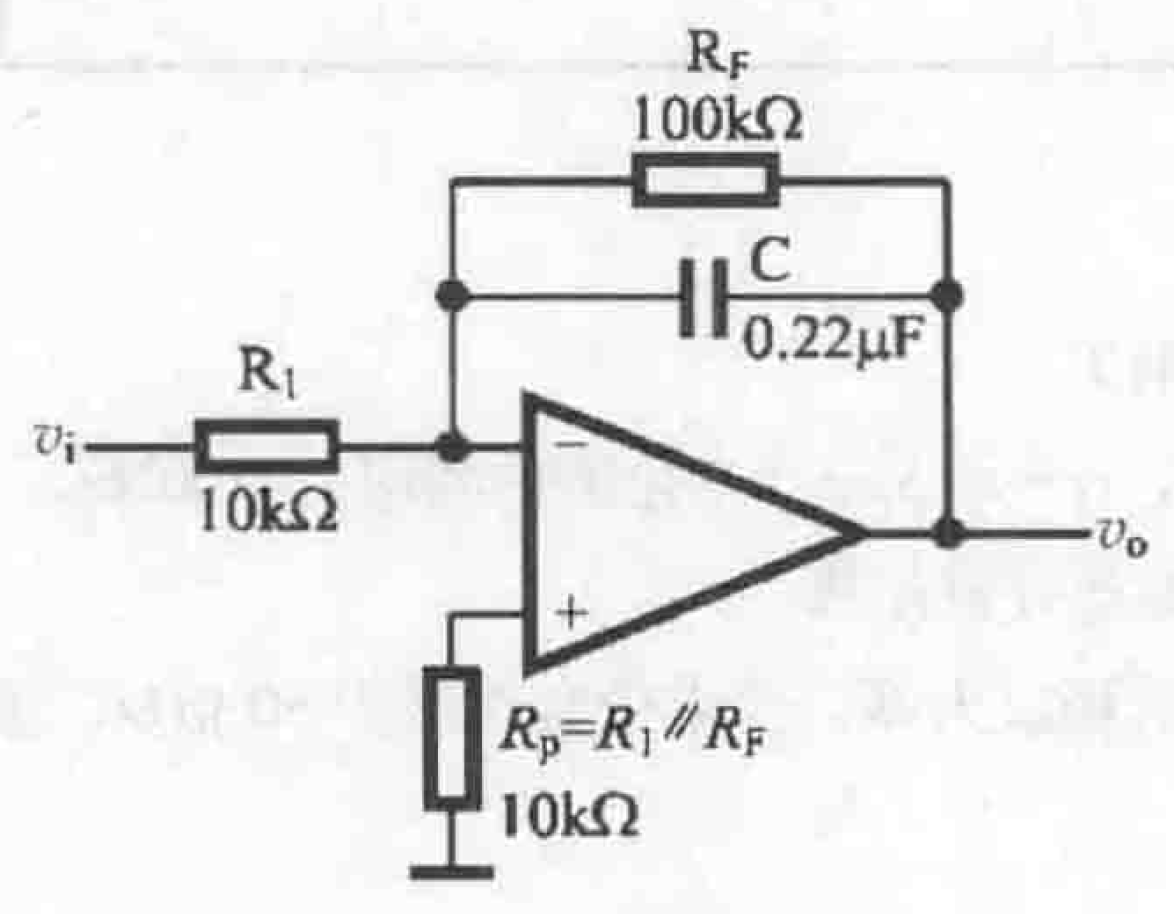
\includegraphics[scale=0.18]{1.4}
	\caption*{任务3: 比例积分电路测试}
\end{figure}
从信号源送出 200Hz、1V 的正方波作为 $v_\mathrm{i}$, 用示波器两个通道同时观测$v_\mathrm{i}$和$v_\mathrm{o}$,并定量画出它们的波形(需含有坐标轴,波形上下对齐)
\section{实验数据分析}
\subsection{任务1: 研究电压跟随器的作用}
观察到的波形如下:
\begin{figure}[H]
	\centering
	\setcounter{subfigure}{0}
	\subfigure[不接入$R_L$]{
		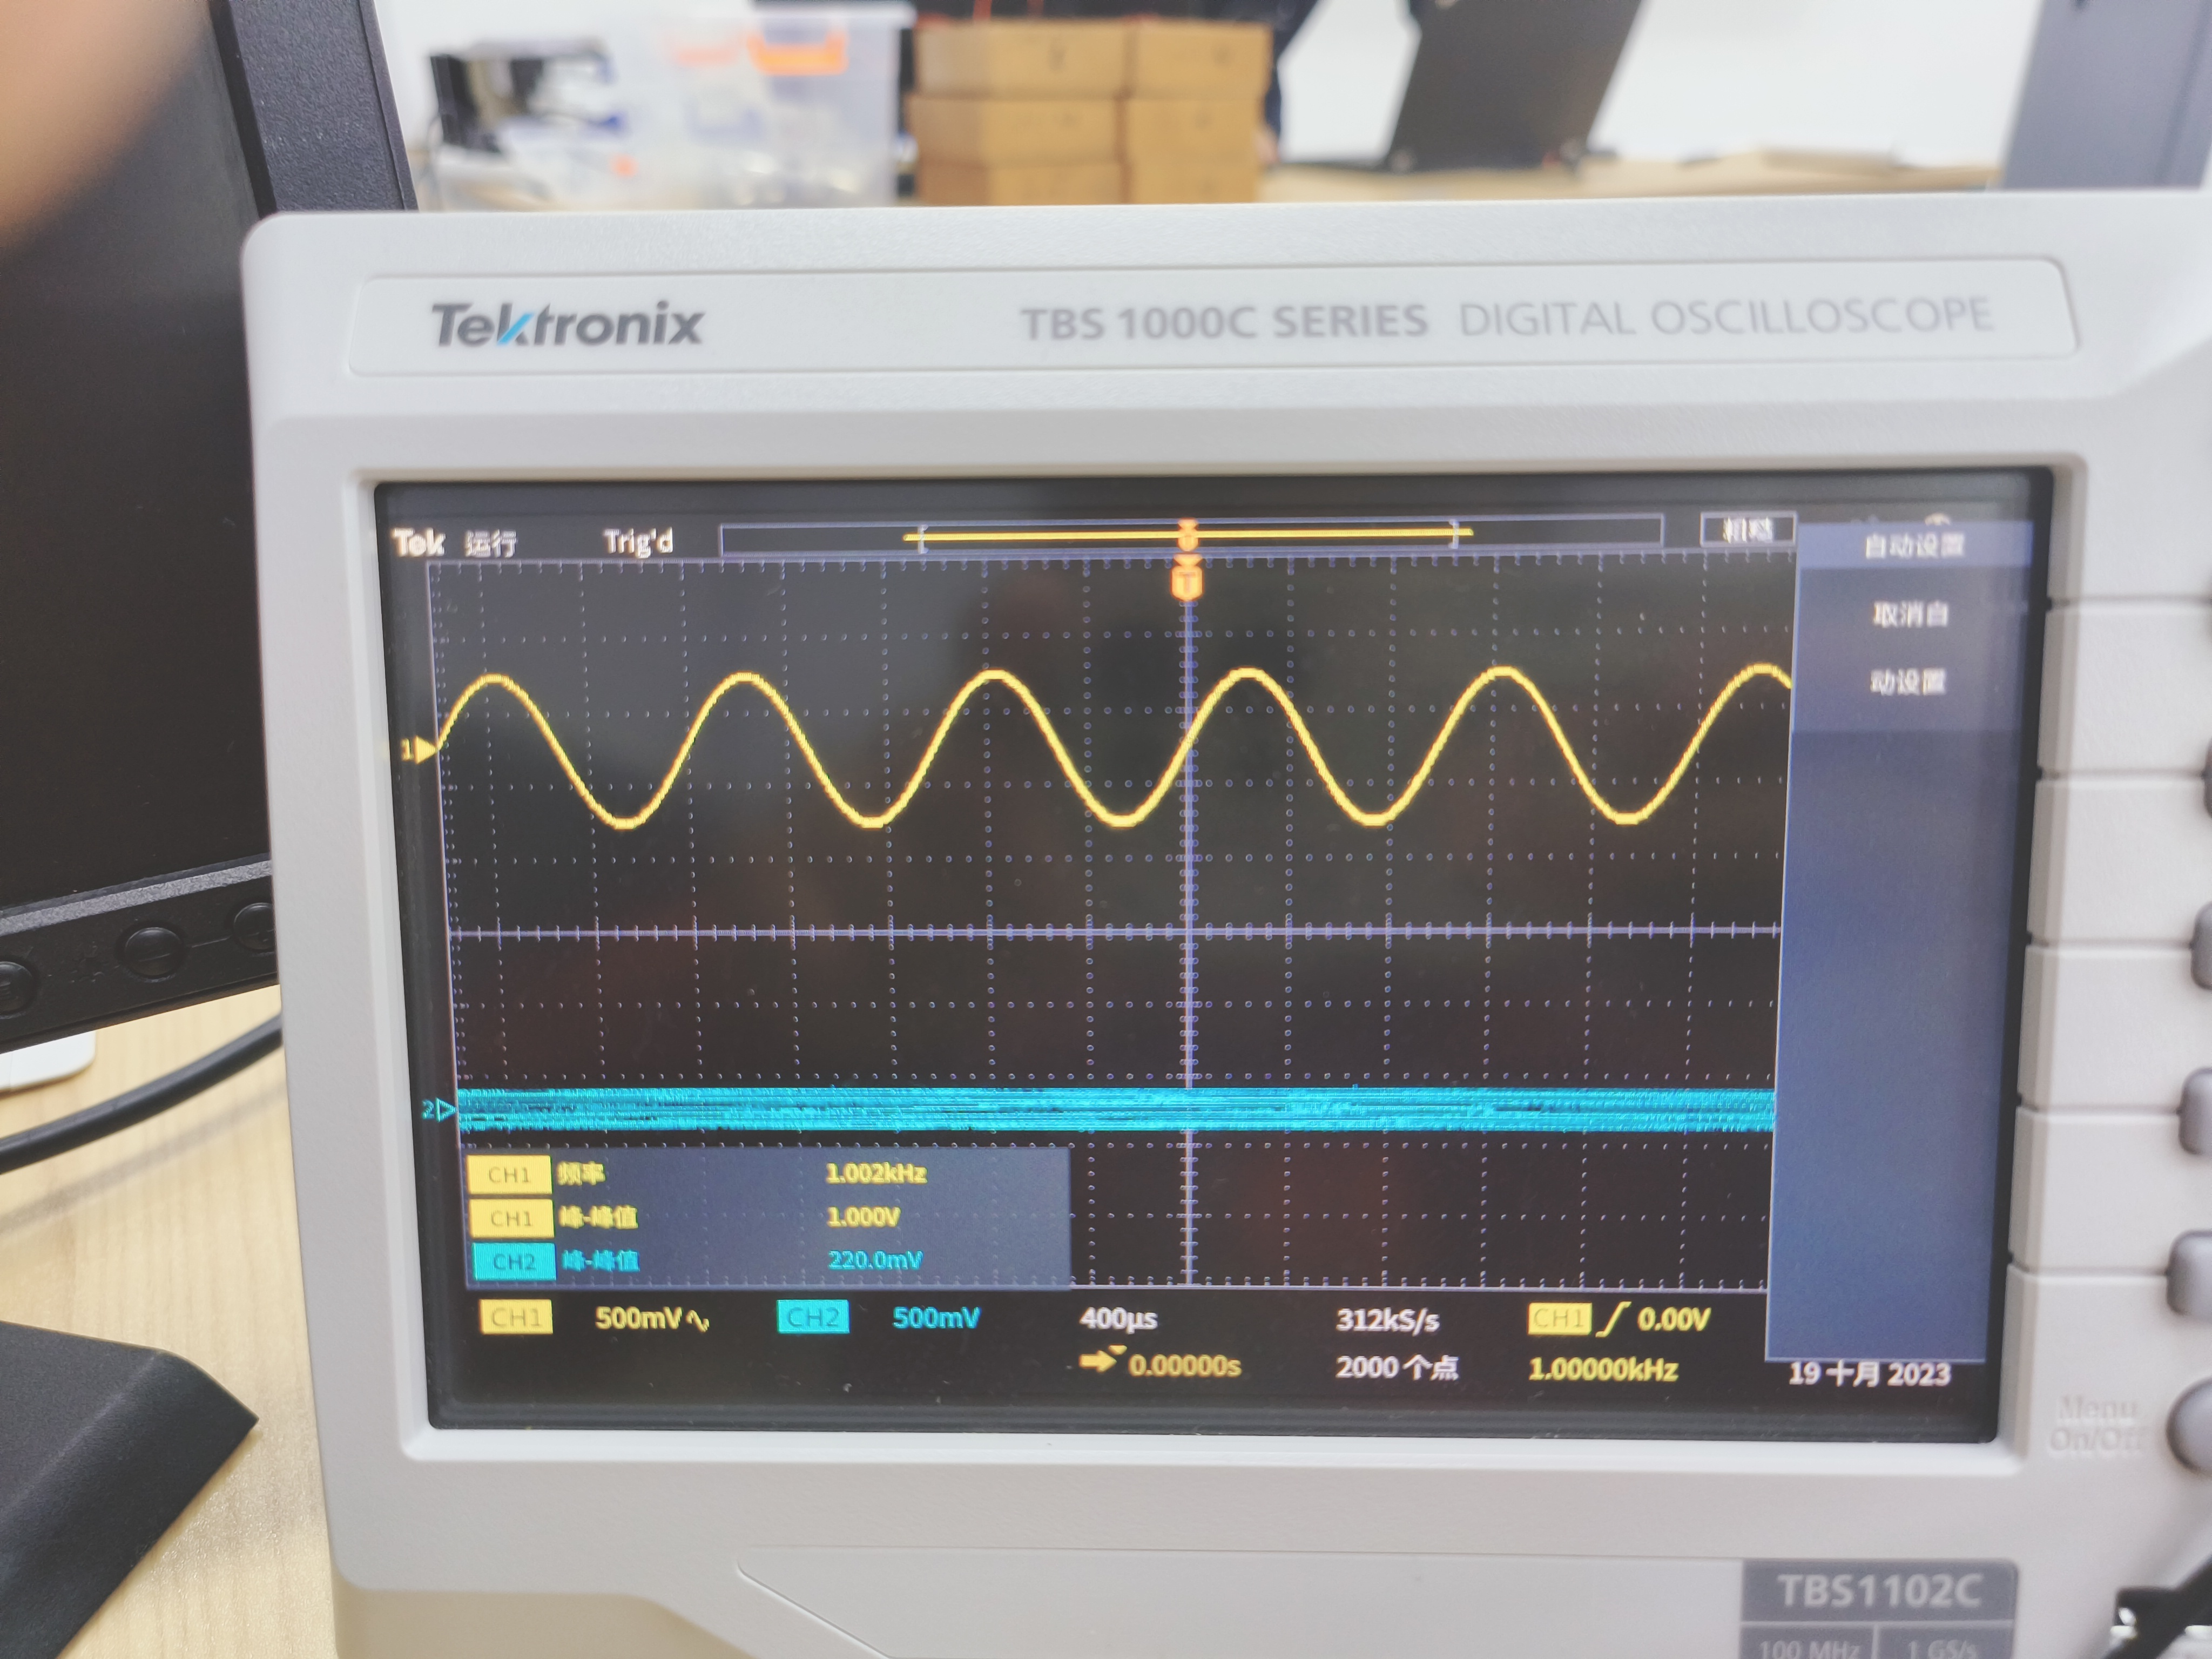
\includegraphics[width=0.48\textwidth]{1.5}
	}
	\subfigure[接入$R_L$]{
		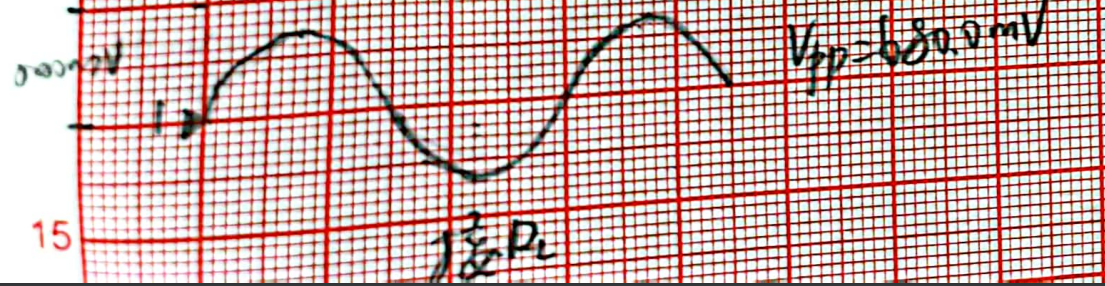
\includegraphics[width=0.48\textwidth]{1.6}
	}
	
	\caption*{无信号跟随器}
\end{figure}

\begin{figure}[H]
	\centering
	\setcounter{subfigure}{0}
	\subfigure[不接入$R_L$]{
		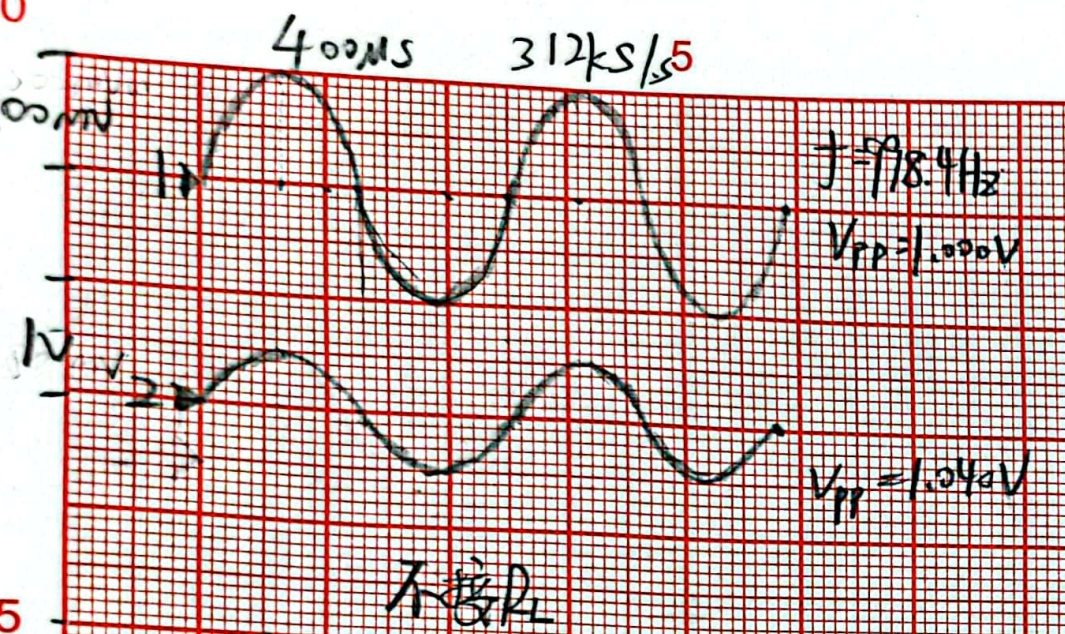
\includegraphics[width=0.48\textwidth]{1.7}
	}
	\subfigure[接入$R_L$]{
		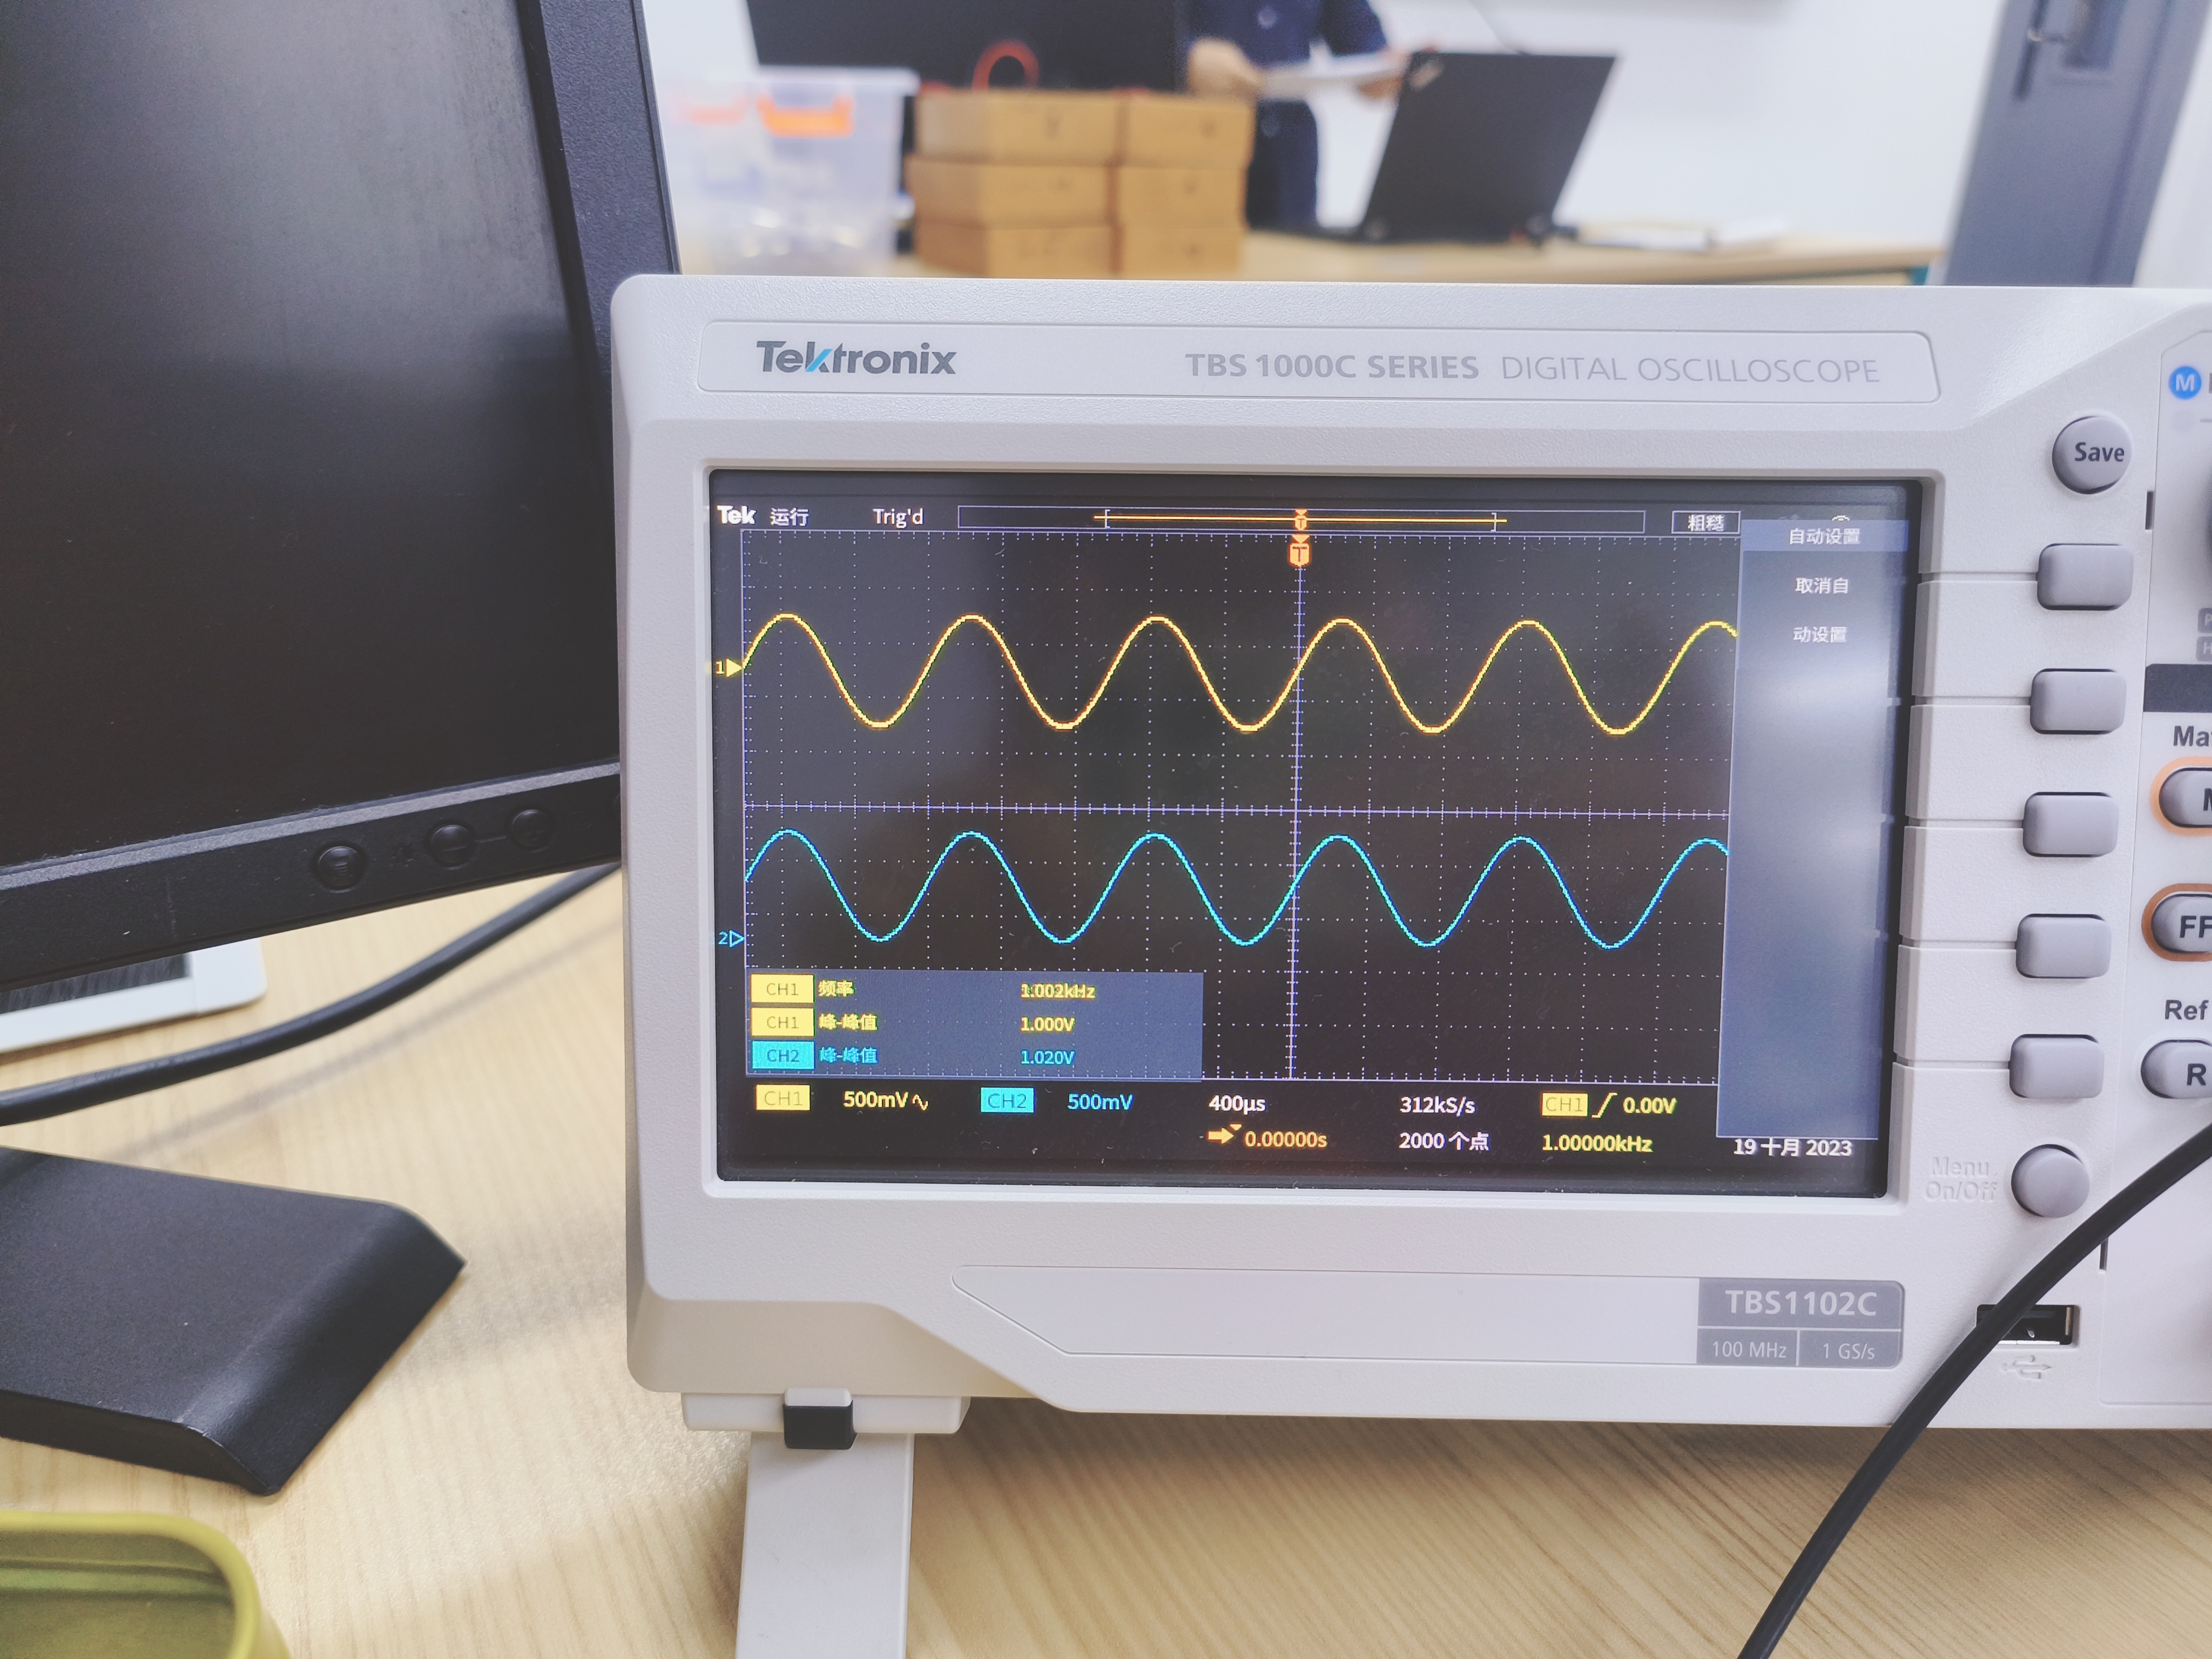
\includegraphics[width=0.48\textwidth]{1.8}
	}
	
	\caption*{有信号跟随器}
\end{figure}
可以看到在缺少电压跟随器时,接入$R_L$后电压下降明显,并根据分压公式计算出了信号源内阻。负载效应是指由于负载电阻的存在,导致信号源输出电压产生电压降。由于负载电阻的存在,信号源的输出电压会在连接负载时产生降低。根据欧姆定律,当电流经过电阻时,会产生电压降。因此,连接100Ω负载电阻后,信号源输出电压会相应降低。
\newpage
数据记录表格如下:
\begin{figure}[H]
	\centering
	\caption*{电压跟随器数据记录表格}
	
	\begin{tabular}{|c|c|c|c|c|c|}
		\hline
		\multirow{2}{*}{}   & \multicolumn{2}{c|}{不接$R_L$} & \multicolumn{2}{c|}{接入$R_L$} &
		\multirow{2}{*}{计算$R_s/\Omega$}\\
		\cline{2-5}
		\multirow{2}{*}{} & $v_{ipp}/$V & $v_{opp}/$V & $v_{ipp}/$V & $v_{opp}/$V & \multirow{2}{*}{}\\
		\hline
		无电压跟随器 & 1.000 & - & 0.6800 & - & 47.06\\
		\hline
		有电压跟随器 & 1.000 & 1.020 & 1.000 & 1.040 & - \\
		\hline
	\end{tabular}
\end{figure} 

\subsection{任务2: 反相比例加法运算电路测试}
实验数据如下,误差在5\%~6\%左右,属于比较合理的实验误差:
\begin{table*}[htbp]
	\centering
	\caption*{加法器实验数据表格}
	\begin{tabular}{|c|c|c|c|c|c|}
		\hline
		\multirow{2}{*}{}   & \multicolumn{3}{c|}{实测值} & 理论值 &
		\multirow{2}{*}{相对误差}\\
		\cline{2-5}
		\multirow{2}{*}{} & $v_{1pp}$/mV & $v_{2pp}/$/mV & $v_{opp}$/V & $v_{opp}$/V & \multirow{2}{*}{}\\
		\hline
		$R_{s2}=1\mathrm{k\Omega}$ & 304.0 & 146.0 & 5.600 & 5.953 & 5.930\% \\
		\hline
		$R_{s2}=500\mathrm{\Omega}$ & 304.0 & 104.0 & 4.800 & 5.125 & 6.341\% \\
		\hline
		实测电阻值 & \multicolumn{5}{c|}{$R_1=9.7813\mathrm{k\Omega},R_2=5.0152\mathrm{k\Omega}, R_F=98.905\mathrm{k\Omega}$}\\
		\hline
	\end{tabular}
\end{table*}

观察到的波形如下(只记录了$R_{s2}=1\mathrm{k\Omega}$的波形):
\begin{figure}[H]
	\centering
	\setcounter{subfigure}{0}
	\subfigure[$v_{1pp}$]{
		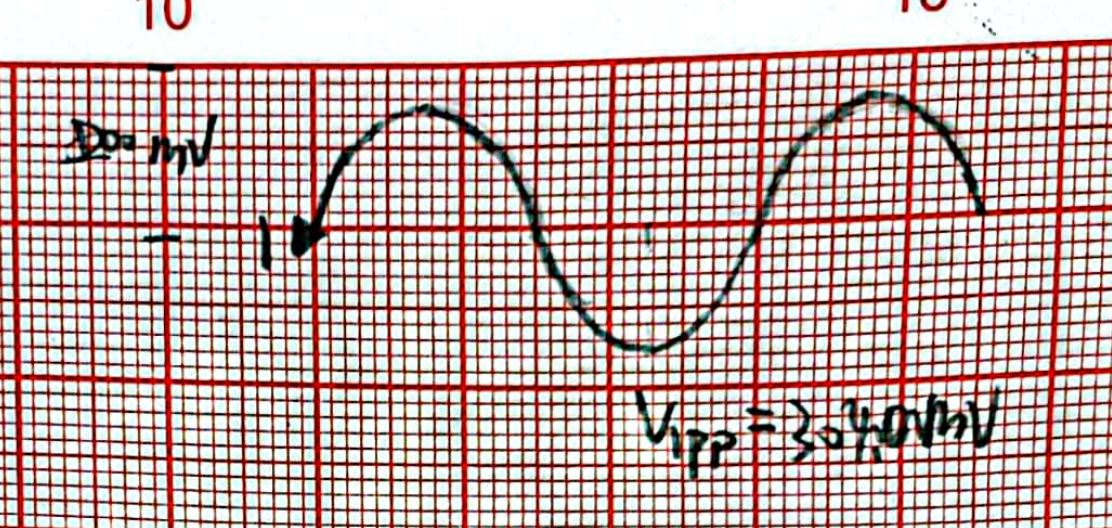
\includegraphics[width=0.3\textwidth]{1.9}
	}
	\subfigure[$v_{2pp}$]{
		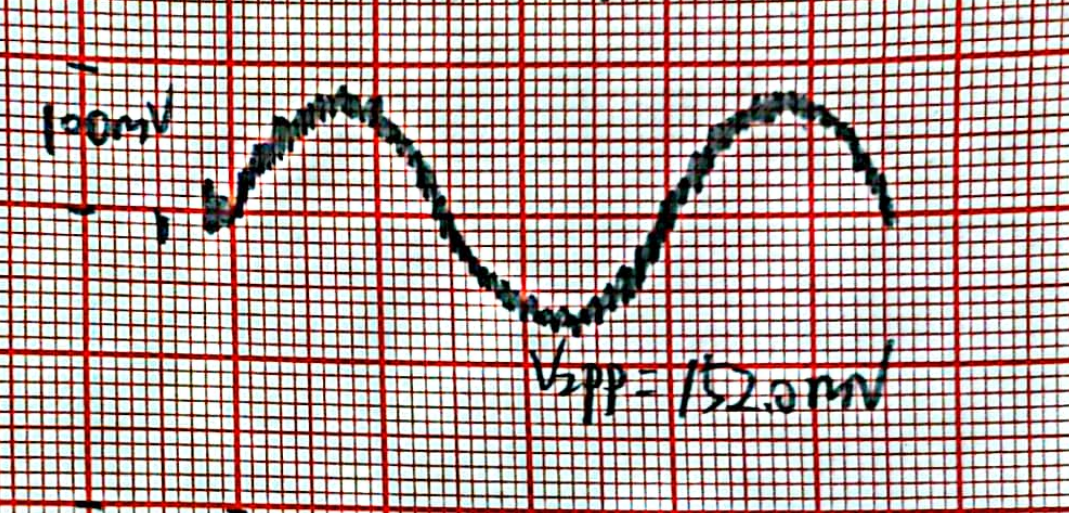
\includegraphics[width=0.3\textwidth]{1.10}
	}
	\subfigure[$v_{opp}$]{
		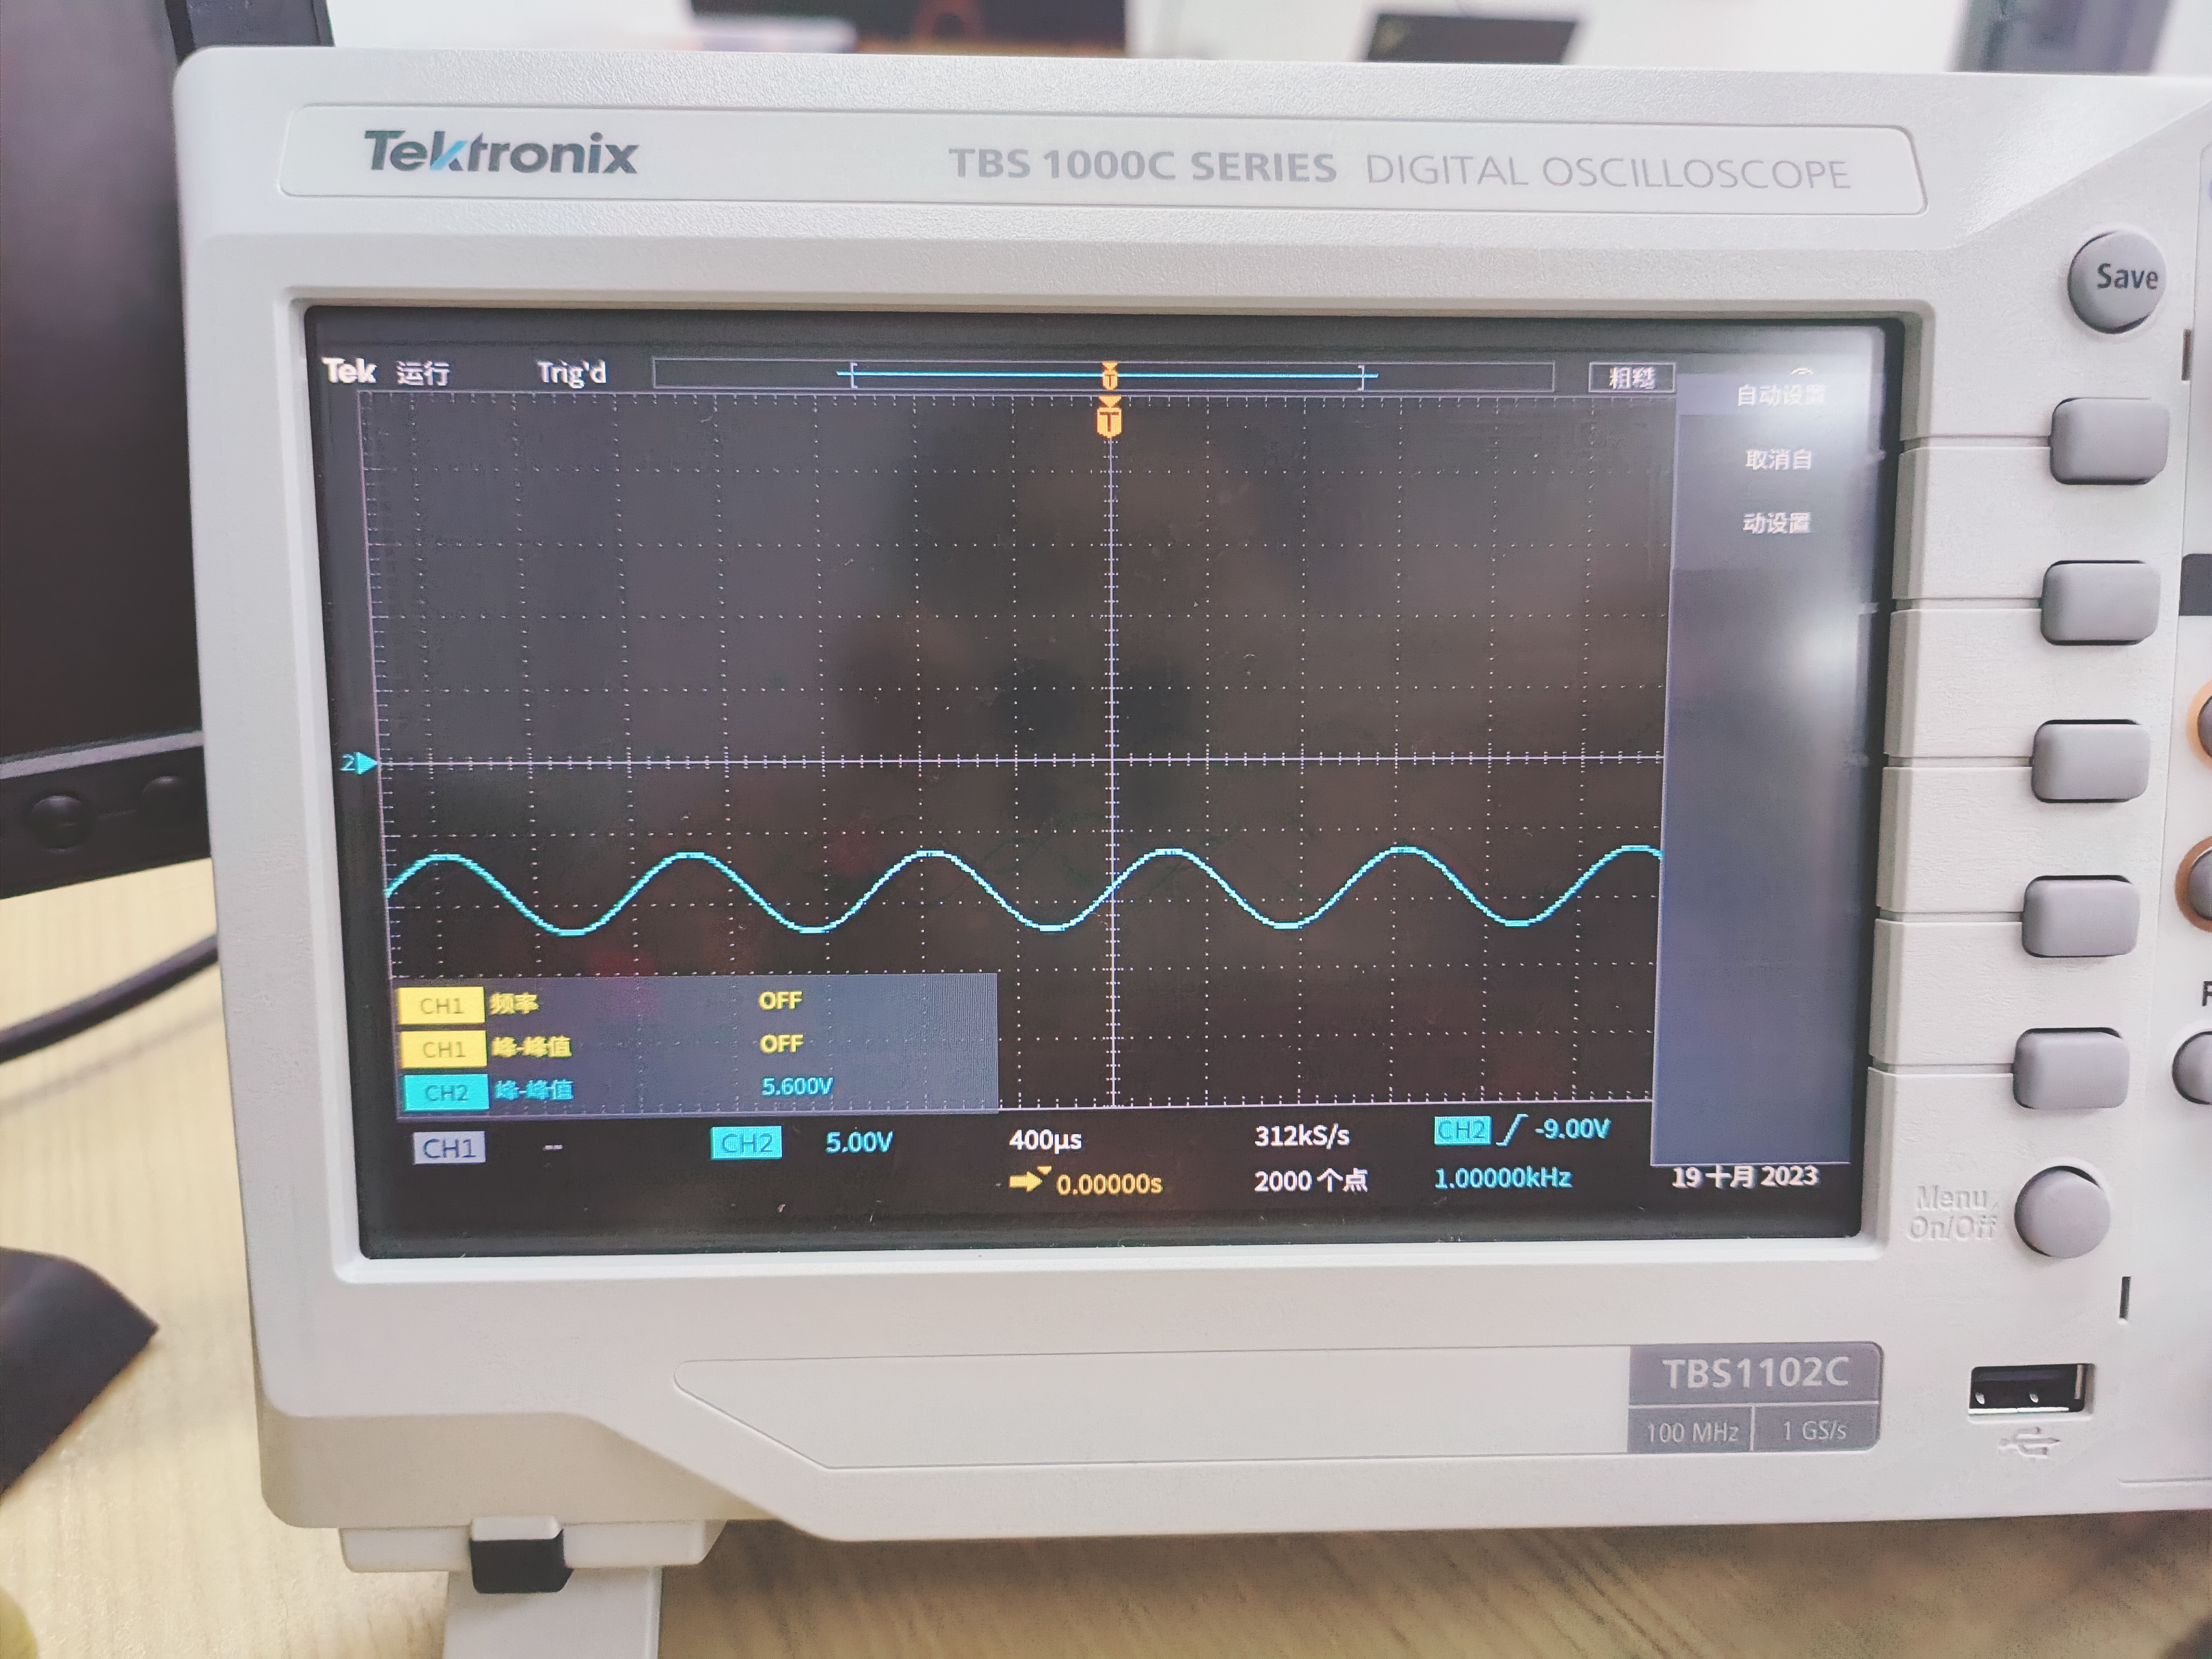
\includegraphics[width=0.3\textwidth]{1.11}
	}
	\caption*{加法器波形图}
\end{figure}
\subsection{任务3: 比例积分电路测试}
观察到的波形如下,基本符合要求:
\begin{figure}[H]
	\centering
	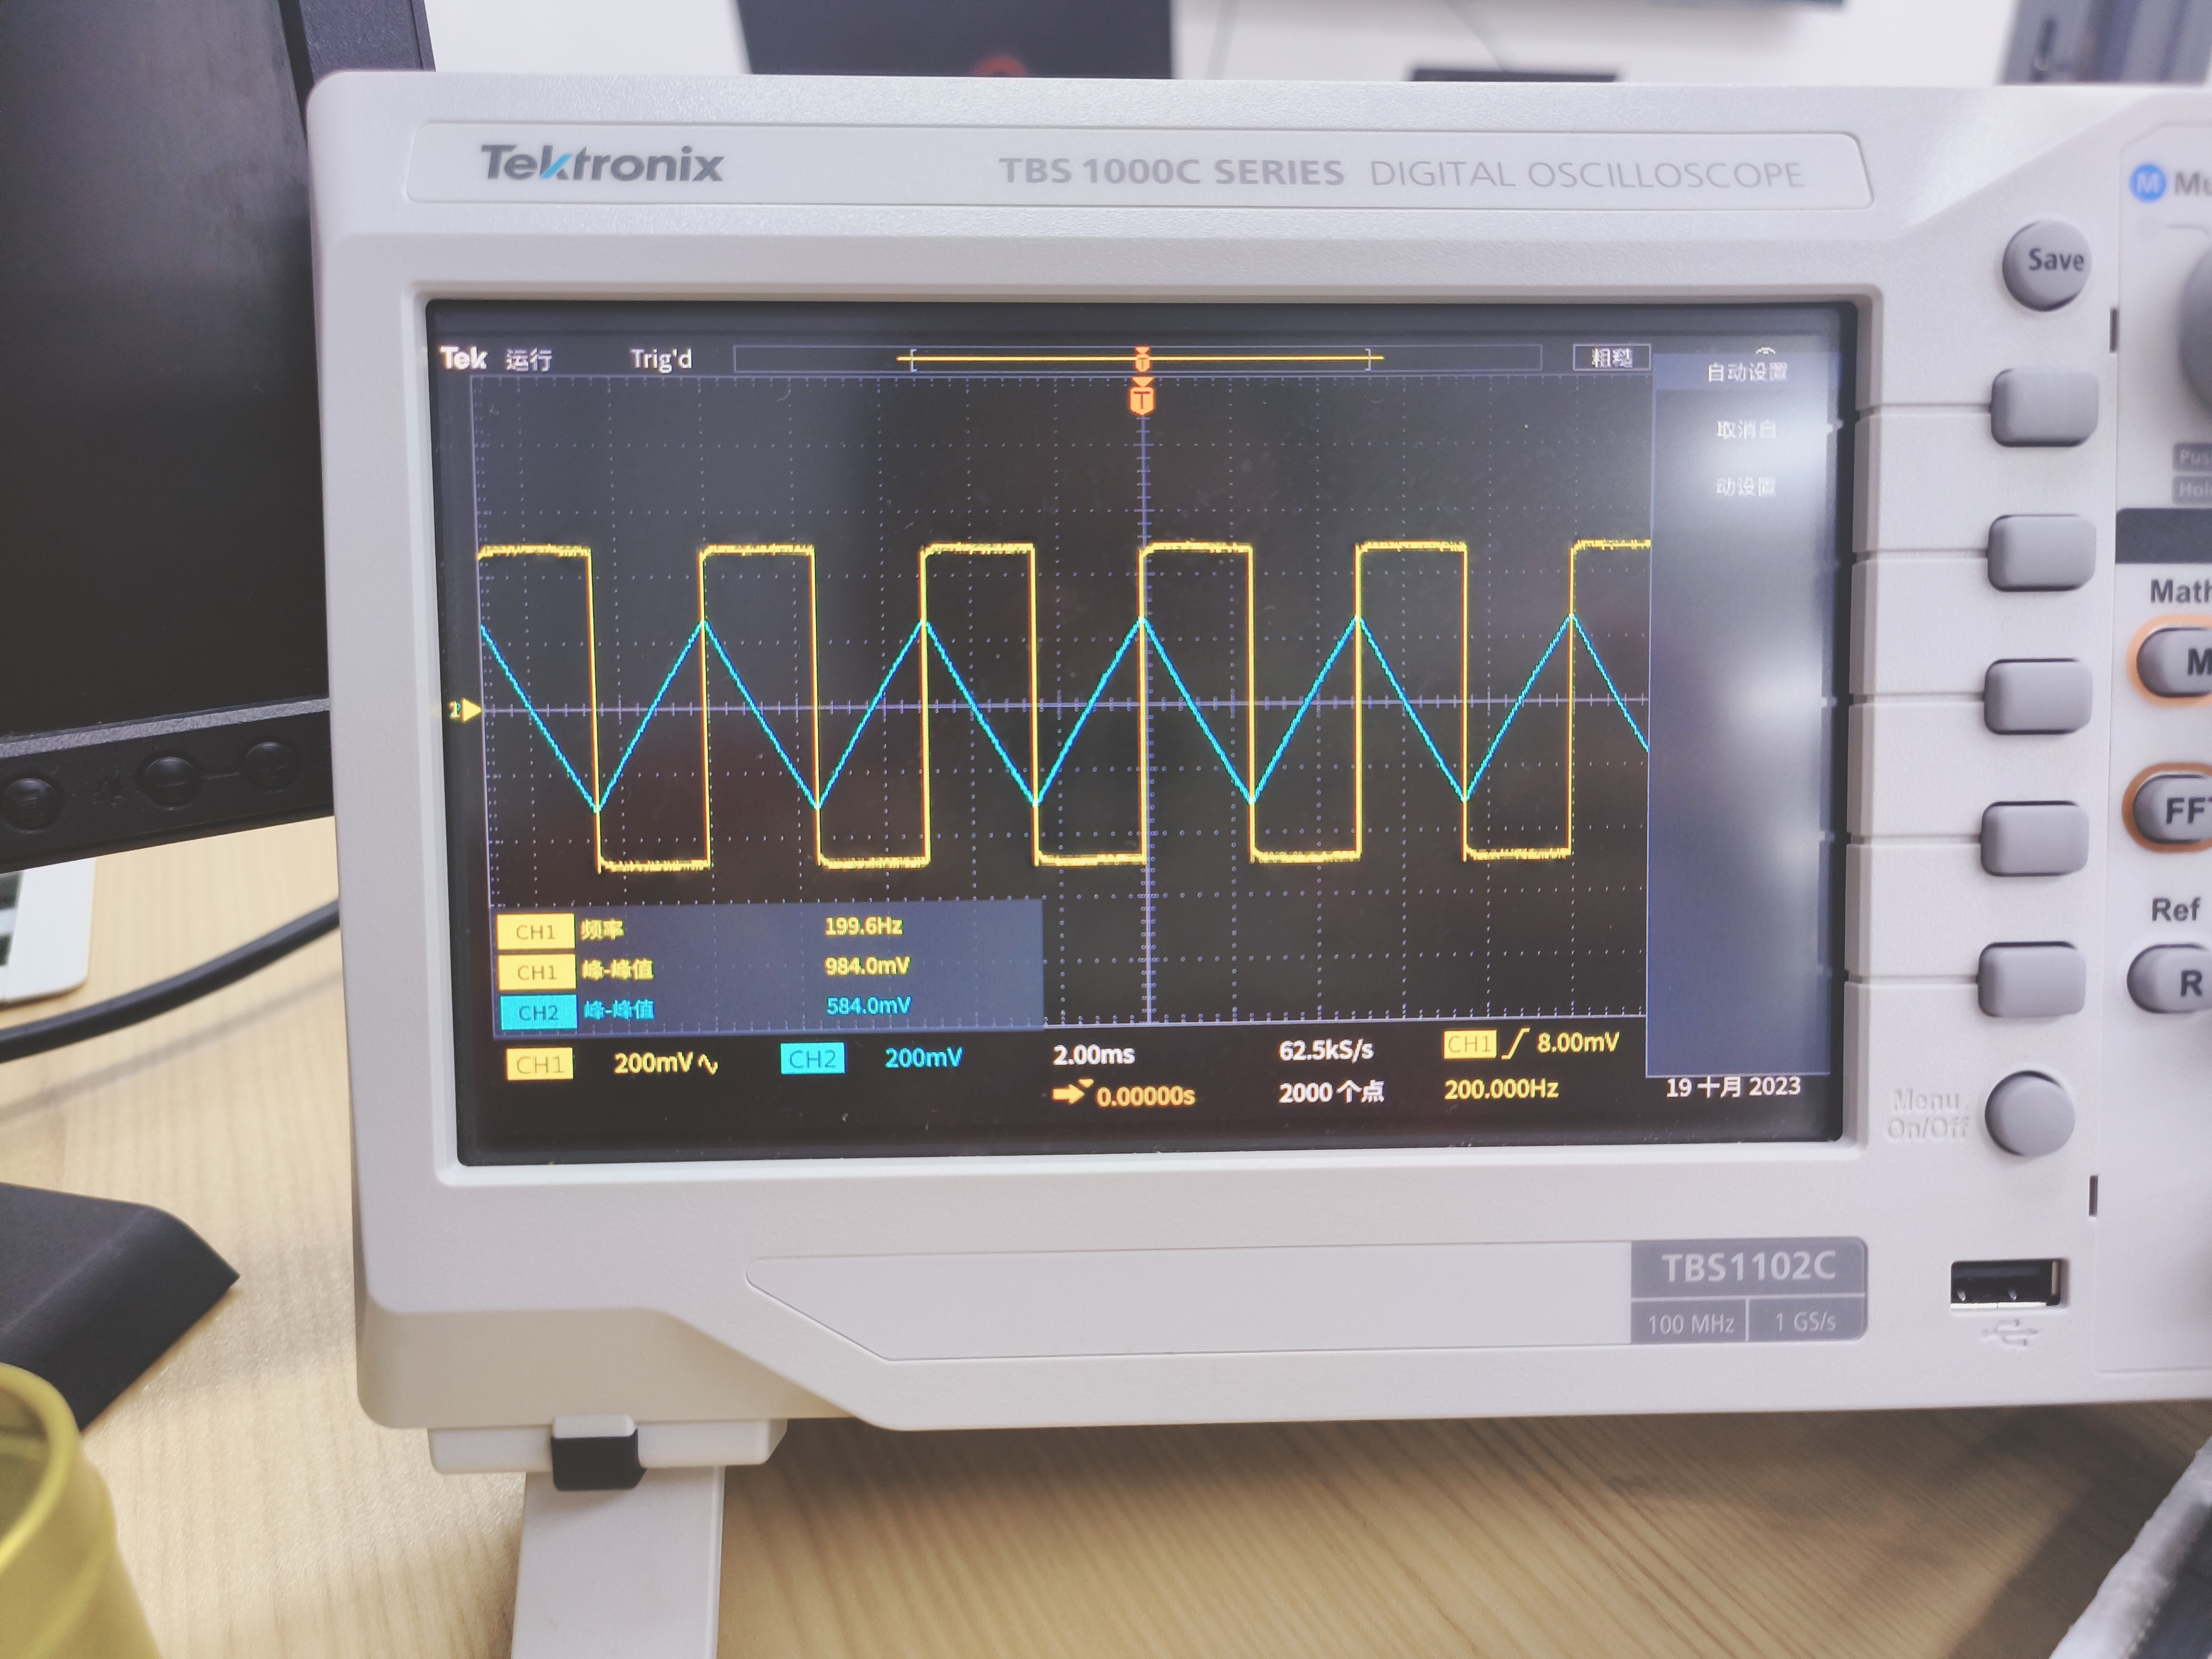
\includegraphics[width=0.7\textwidth]{1.12}
	\caption*{比例积分电路}
\end{figure}
\section{心得、体会与反思}
本次实验是我的第一次模电实验,学会了实验室中信号源、示波器、电源的使用方法,基本掌握了运算放大器NE5532的使用原理和接线方法,基本完成了实验要求。

但是本次实验中也出现了比较严重的实验操作失误:在任务2中,输出信号$v_o$应该用示波器直接测量即可,但是我误将其输出信号接地后再测量,这个操作使得电路产生了极大的电流,造成运放大量积热,所幸实验时我将手指放在运放上(实际上这个操作也有安全隐患),一感受到温度上升便立刻切断了运放的供电电源,并未造成安全事故,这次的教训也提醒我要仔细检查电路的连接方式,不能再次出现这次实验中的错误操作!
\end{document}